\begin{frame}[allowframebreaks]
\frametitle{ggplot2}
\texttt{ggplot2} é um pacote de visualização de dados para R.

\vspace{3ex}
O \texttt{ggplot2} fornece um esquema de visualização de dados que se
utiliza de camadas de conteúdo semântico. Os dados devem ser dispostos em \emph{dataframes} 
ao invés de vetores individuais.

\framebreak 

O \texttt{ggplot2} é diferente de outros pacotes de visualização pois ele
possui uma gramática subjacente.

\vspace{3ex}
Ele é baseado na Gramática de Gráficos proposta por \textcite{wilkinson2005grammar}.

\vspace{3ex}
Uma gramática de uma língua a torna expressiva. Ao especificar a relação entre palavras em um sentença
uma gramática expande o escopo da língua além de meras palavras isoladas.

\vspace{3ex}
Uma gramática de gráficos permite ir além de gráficos (palavras), expandindo nosso horizonte a formas
gráficas mais complexas (sentenças). As regras desta gramática podem ter natureza matemática ou estética.
\end{frame}


\begin{frame}
\frametitle{Especificação de gráficos}

A especificação de gráficos passa por seis etapas \cite{wilkinson2005grammar}:
\begin{enumerate}
\item \textbf{Dados} (\emph{dataset})
\item \textbf{Transformação} de variáveis (ex.: ordenamento)
\item \textbf{Escala} (ex.: logaritmo)
\item \textbf{Coordenadas} (ex.: cartesianas, polar)
\item \textbf{Elementos} gráficos (ex.: pontos, linhas, barras) e seus atributos estéticos (ex.: cor)
\item \textbf{Guias} (ex.: eixos, legendas)
\end{enumerate}

\end{frame}

\begin{frame}[fragile,allowframebreaks]
\frametitle{ggplot2 - wine quality data set}
\centering

\lstinputlisting[language=R, label=lst-ggplotwine-1, firstline=1, lastline=6, postbreak=\mbox{$\hookrightarrow$\space}, basicstyle=\fontsize{8}{10}\selectfont\ttfamily]{examples/ggplot-wine.r}

\framebreak
\lstinputlisting[language=R, label=lst-ggplotwine-2, firstline=7, lastline=28, postbreak=\mbox{$\hookrightarrow$\space}, basicstyle=\fontsize{8}{10}\selectfont\ttfamily]{examples/ggplot-wine.r} 

\framebreak
\lstinputlisting[language=R, label=lst-ggplotwine-3, firstline=29, lastline=34, postbreak=\mbox{$\hookrightarrow$\space}, basicstyle=\fontsize{8}{10}\selectfont\ttfamily]{examples/ggplot-wine.r} 

\framebreak
\lstinputlisting[language=R, label=lst-ggplotwine-4, firstline=36, lastline=38, postbreak=\mbox{$\hookrightarrow$\space}, basicstyle=\fontsize{8}{10}\selectfont\ttfamily]{examples/ggplot-wine.r} 
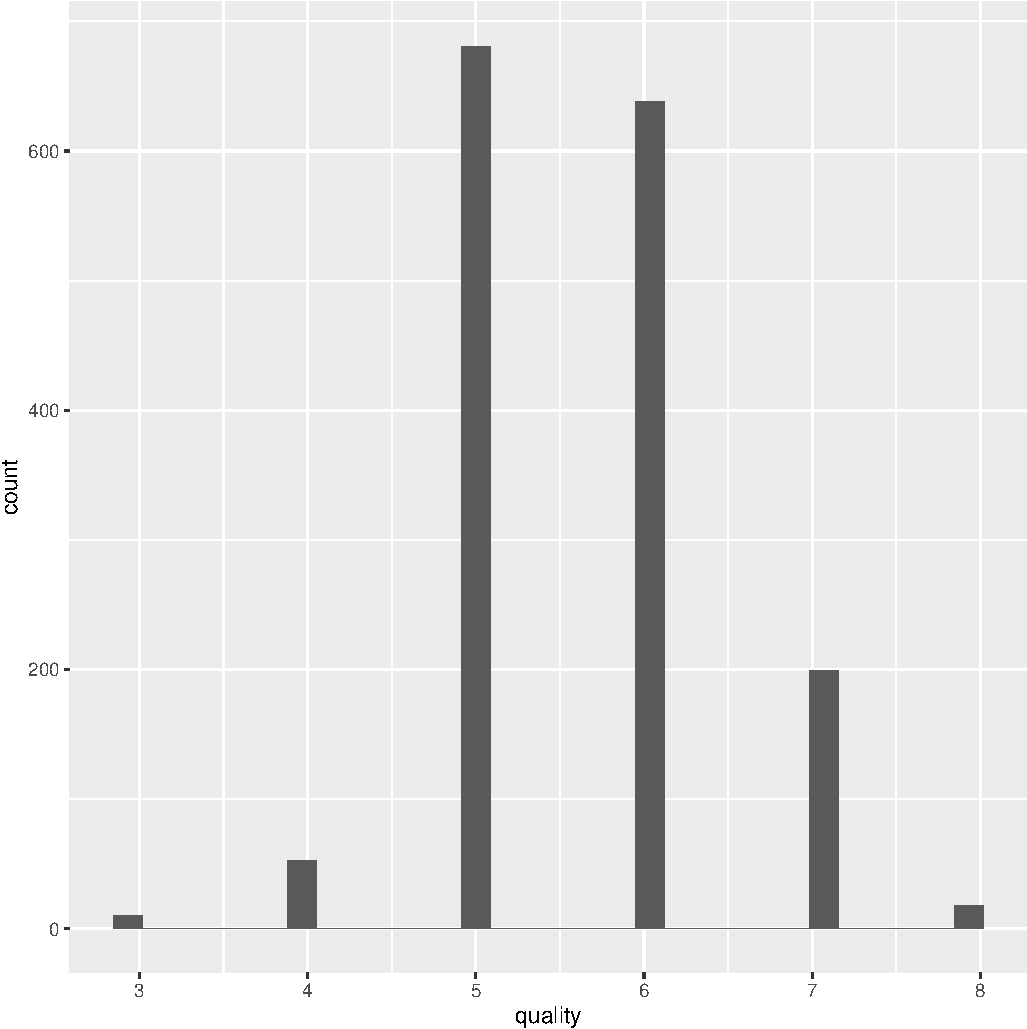
\includegraphics[width=0.8\textwidth,height=0.7\textheight,keepaspectratio]{examples/ex-ggplot-01-crop.pdf}

\framebreak
\lstinputlisting[language=R, label=lst-ggplotwine-5, firstline=39, lastline=40, postbreak=\mbox{$\hookrightarrow$\space}, basicstyle=\fontsize{8}{10}\selectfont\ttfamily]{examples/ggplot-wine.r} 
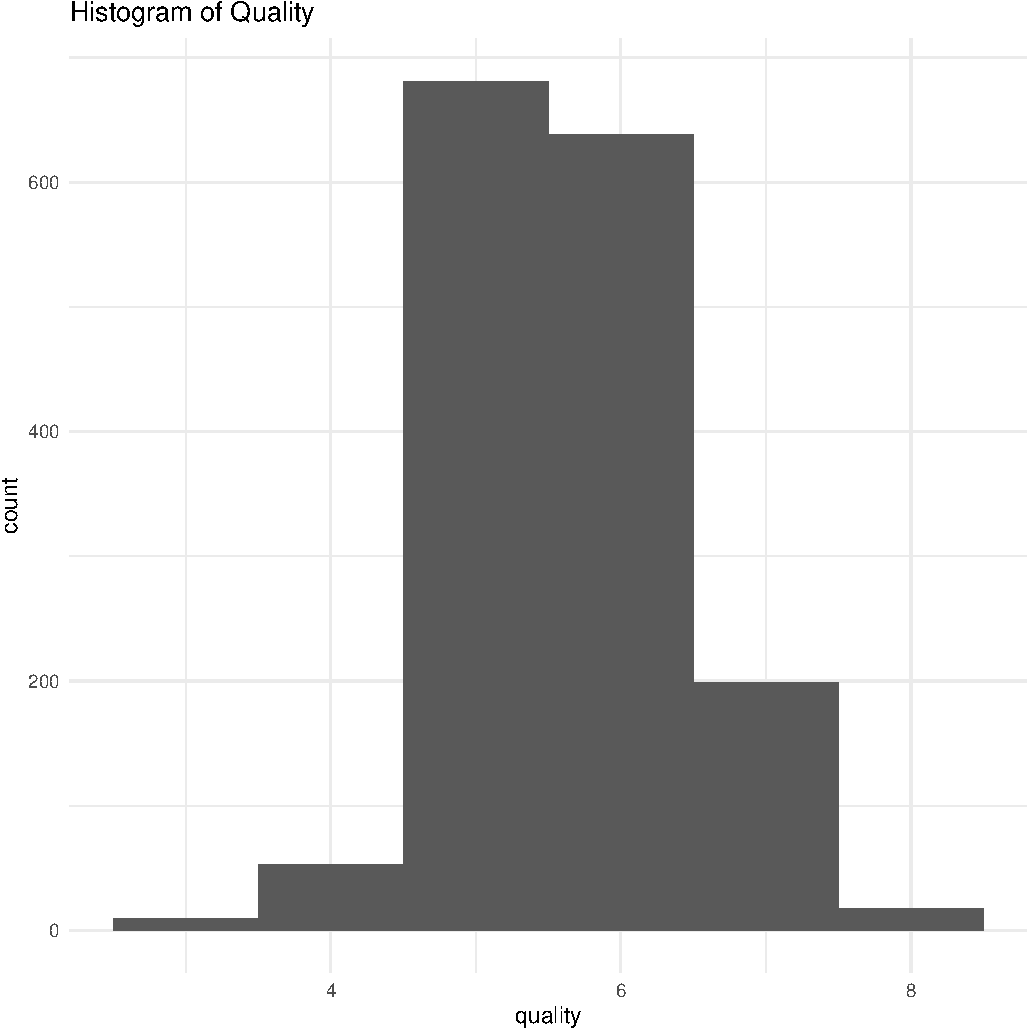
\includegraphics[width=0.8\textwidth,height=0.7\textheight,keepaspectratio]{examples/ex-ggplot-02-crop.pdf}

\framebreak
\lstinputlisting[language=R, label=lst-ggplotwine-6, firstline=41, lastline=42, postbreak=\mbox{$\hookrightarrow$\space}, basicstyle=\fontsize{8}{10}\selectfont\ttfamily]{examples/ggplot-wine.r} 
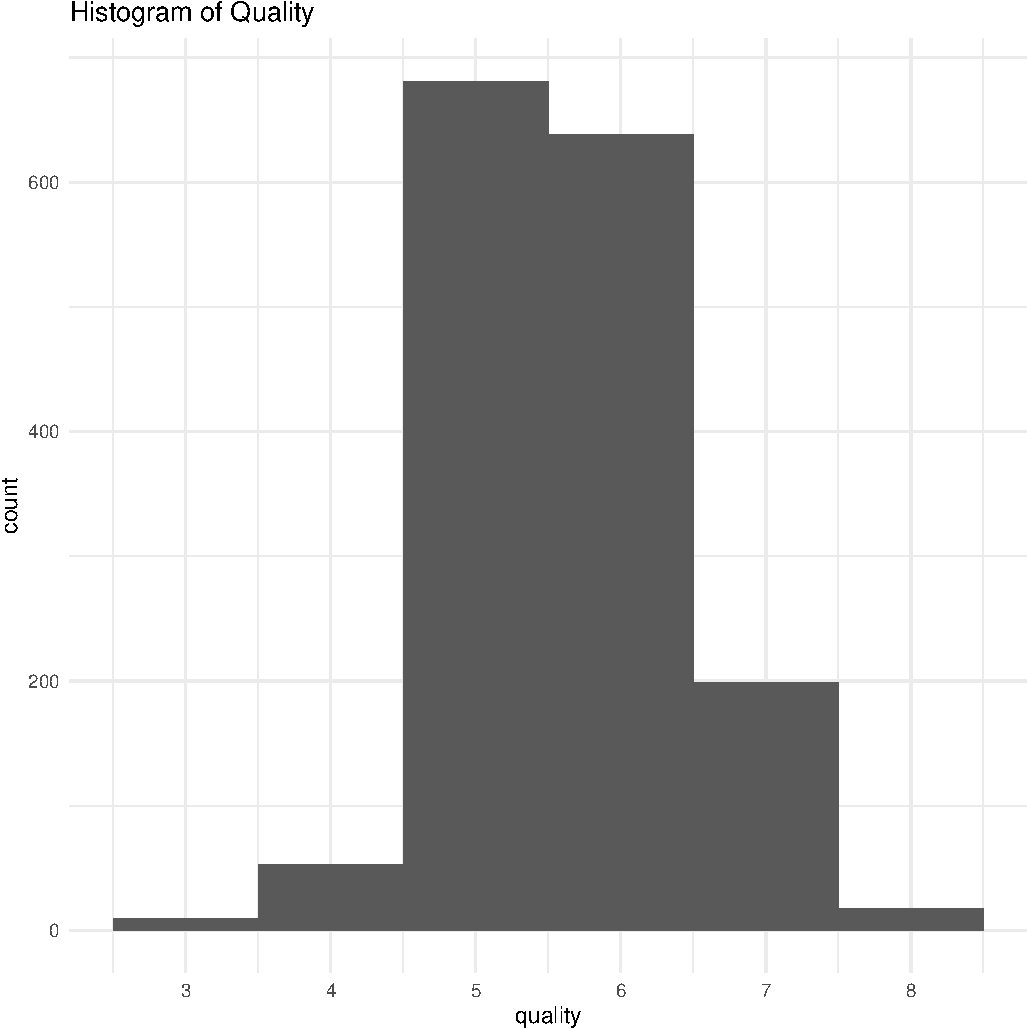
\includegraphics[width=0.8\textwidth,height=0.7\textheight,keepaspectratio]{examples/ex-ggplot-03-crop.pdf}

\framebreak
\lstinputlisting[language=R, label=lst-ggplotwine-7, firstline=43, lastline=44, postbreak=\mbox{$\hookrightarrow$\space}, basicstyle=\fontsize{8}{10}\selectfont\ttfamily]{examples/ggplot-wine.r} 

\includegraphics[width=0.8\textwidth,height=0.7\textheight,keepaspectratio]{examples/ex-ggplot-04-crop.pdf}

\framebreak
\lstinputlisting[language=R, label=lst-ggplotwine-8, firstline=45, lastline=46, postbreak=\mbox{$\hookrightarrow$\space}, basicstyle=\fontsize{8}{10}\selectfont\ttfamily]{examples/ggplot-wine.r} 
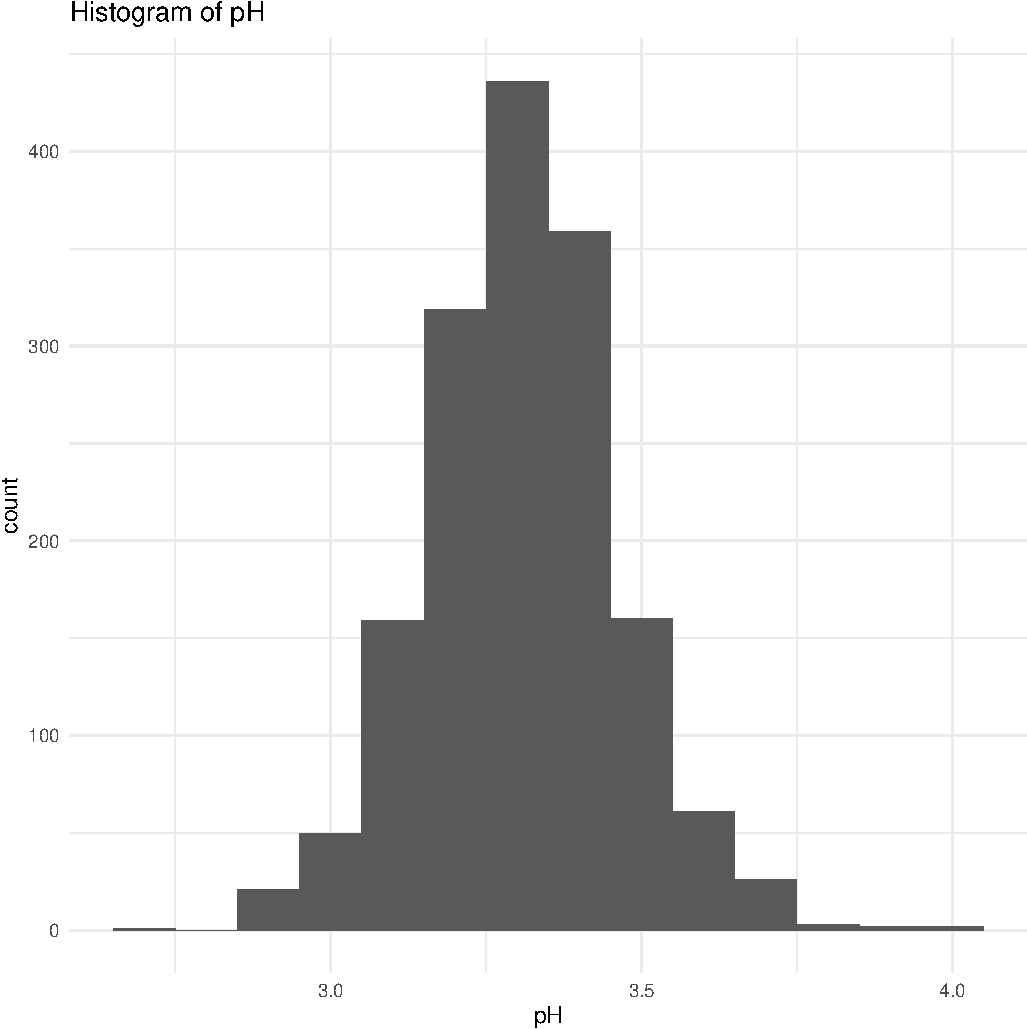
\includegraphics[width=0.8\textwidth,height=0.7\textheight,keepaspectratio]{examples/ex-ggplot-05-crop.pdf}

\framebreak
\lstinputlisting[language=R, label=lst-ggplotwine-9, firstline=47, lastline=48, postbreak=\mbox{$\hookrightarrow$\space}, basicstyle=\fontsize{8}{10}\selectfont\ttfamily]{examples/ggplot-wine.r} 
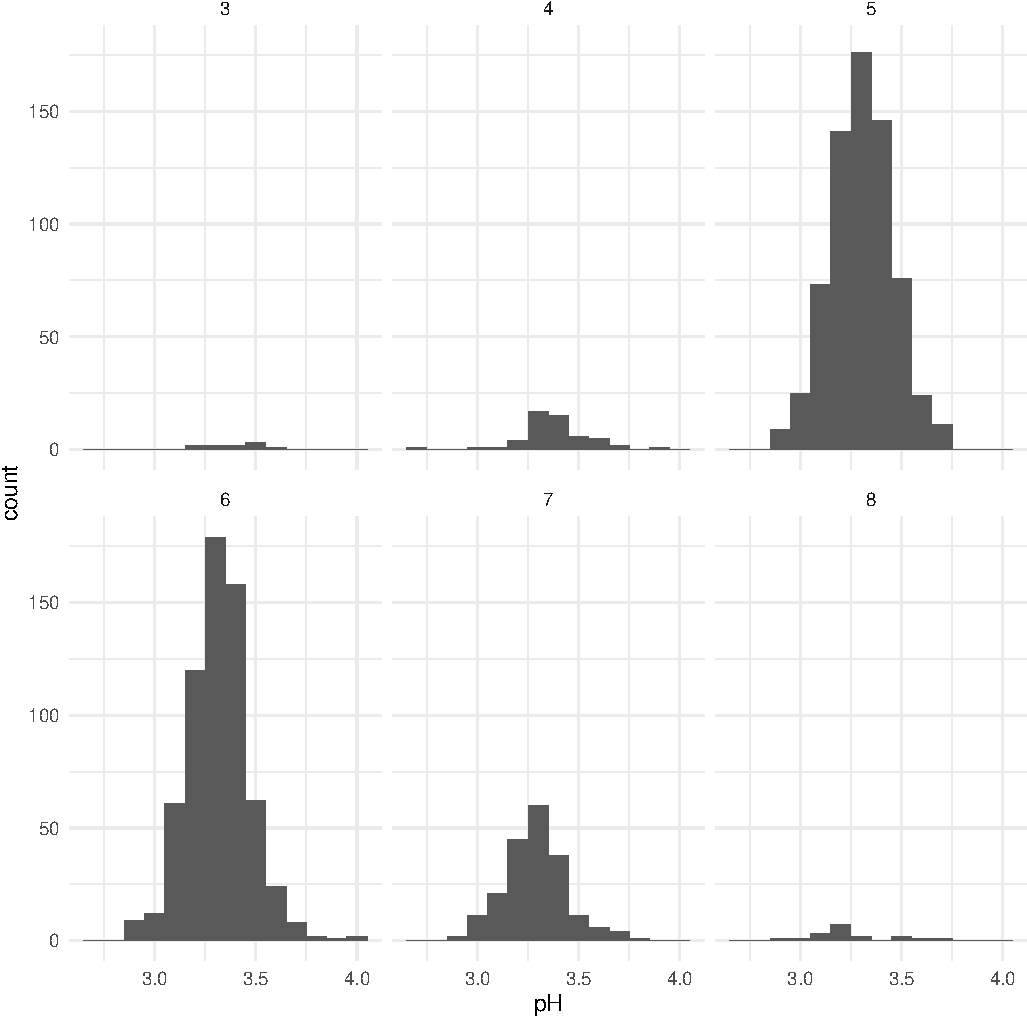
\includegraphics[width=0.8\textwidth,height=0.7\textheight,keepaspectratio]{examples/ex-ggplot-06-crop.pdf}

\framebreak
\lstinputlisting[language=R, label=lst-ggplotwine-10, firstline=49, lastline=50, postbreak=\mbox{$\hookrightarrow$\space}, basicstyle=\fontsize{8}{10}\selectfont\ttfamily]{examples/ggplot-wine.r} 
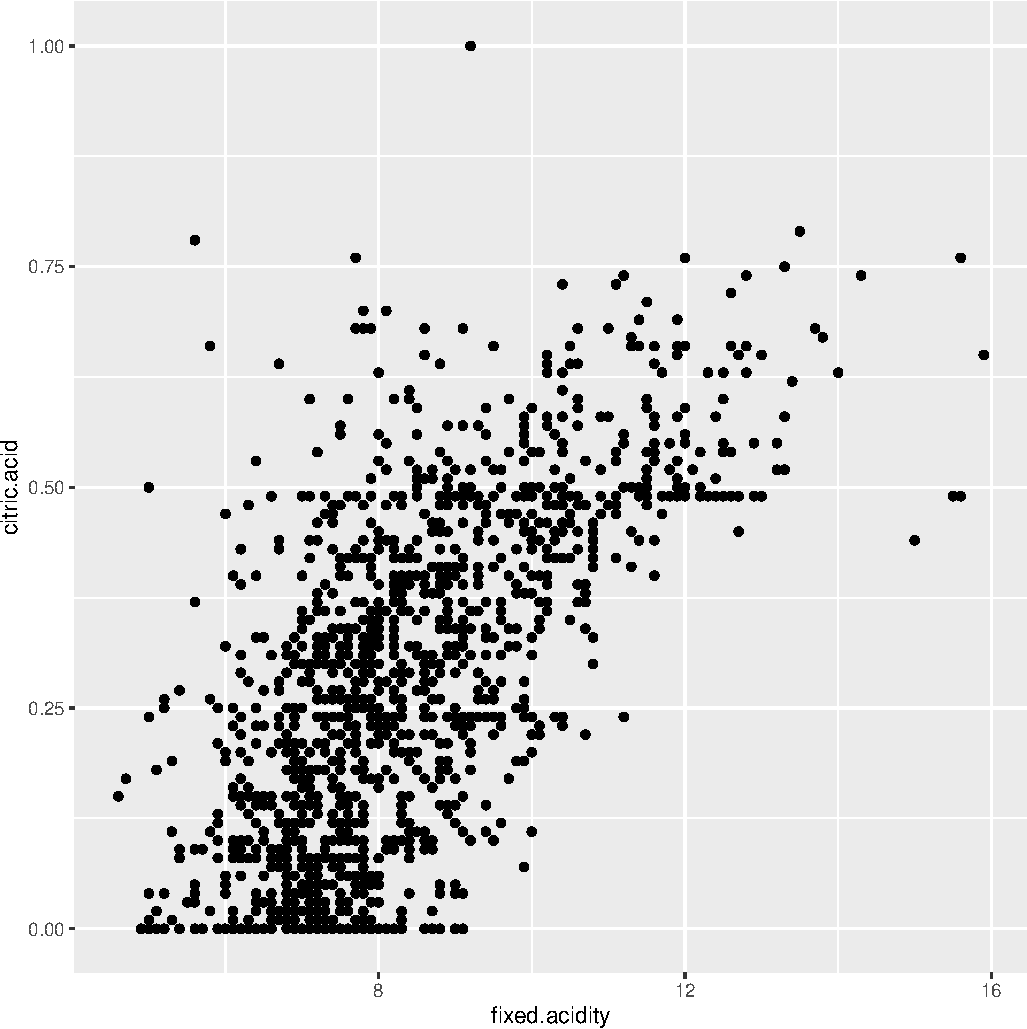
\includegraphics[width=0.8\textwidth,height=0.7\textheight,keepaspectratio]{examples/ex-ggplot-07-crop.pdf}

\framebreak
\lstinputlisting[language=R, label=lst-ggplotwine-11, firstline=51, lastline=52, postbreak=\mbox{$\hookrightarrow$\space}, basicstyle=\fontsize{8}{10}\selectfont\ttfamily]{examples/ggplot-wine.r} 
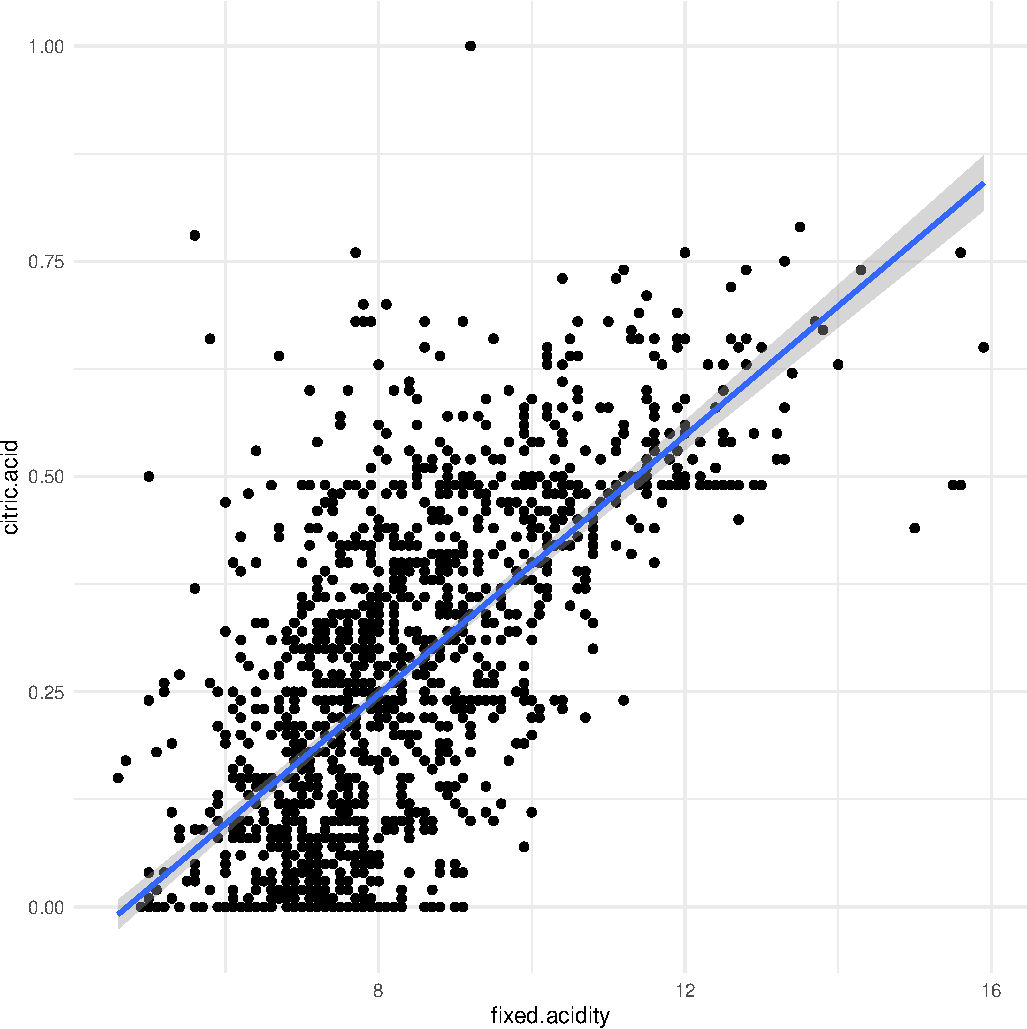
\includegraphics[width=0.8\textwidth,height=0.7\textheight,keepaspectratio]{examples/ex-ggplot-08-crop.pdf}

\framebreak
\lstinputlisting[language=R, label=lst-ggplotwine-12, firstline=53, lastline=54, postbreak=\mbox{$\hookrightarrow$\space}, basicstyle=\fontsize{8}{10}\selectfont\ttfamily]{examples/ggplot-wine.r} 
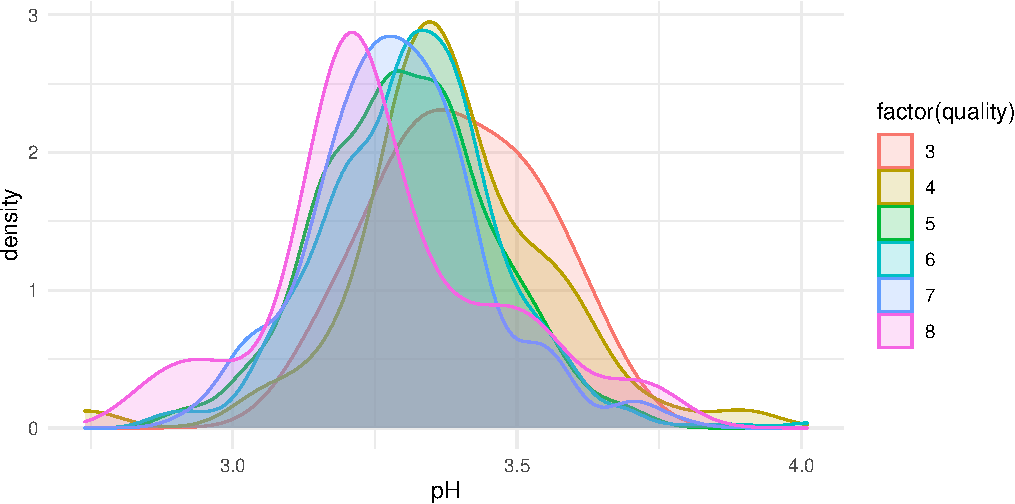
\includegraphics[width=0.8\textwidth,height=0.7\textheight,keepaspectratio]{examples/ex-ggplot-09-crop.pdf}

\framebreak
\lstinputlisting[language=R, label=lst-ggplotwine-13, firstline=55, lastline=56, postbreak=\mbox{$\hookrightarrow$\space}, basicstyle=\fontsize{8}{10}\selectfont\ttfamily]{examples/ggplot-wine.r} 
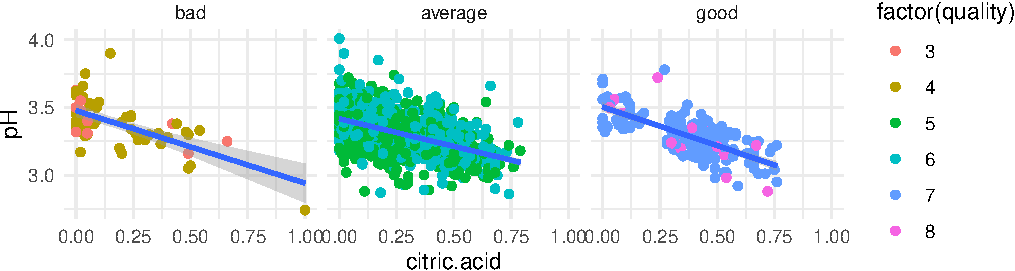
\includegraphics[width=0.8\textwidth,height=0.7\textheight,keepaspectratio]{examples/ex-ggplot-10-crop.pdf}

\framebreak
\lstinputlisting[language=R, label=lst-ggplotwine-14, firstline=57, lastline=58, postbreak=\mbox{$\hookrightarrow$\space}, basicstyle=\fontsize{8}{10}\selectfont\ttfamily]{examples/ggplot-wine.r} 
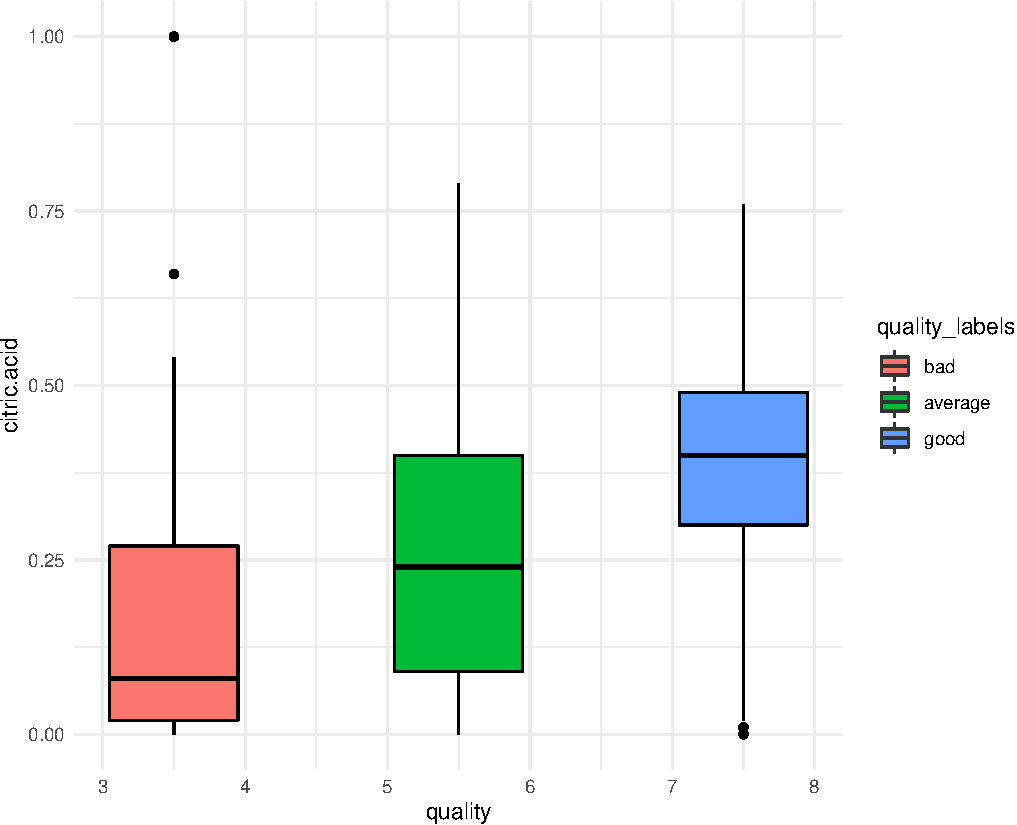
\includegraphics[width=0.8\textwidth,height=0.7\textheight,keepaspectratio]{examples/ex-ggplot-11-crop.pdf}

\end{frame}

%\multido{\i=1+1}{7}{%
%  \begin{frame}[fragile]
%  \frametitle{ggplot2 - example \i}
%  \i
%%  \centering
%%  \lstinputlisting[language=R, label=lst-ggplotwine-\i, firstline=7, lastline=28, postbreak=\mbox{$\hookrightarrow$\space}, basicstyle=\fontsize{8}{10}\selectfont\ttfamily]{examples/ggplot-wine.r}
%%  \includegraphics[width=0.8\textwidth,height=0.7\textheight,keepaspectratio]{figures/ex-ggplot-\ifnum\i<10 0\fi\i.png}
%  \end{frame}
%}


\begin{frame}
\frametitle{Gráficos de mortalidade durante a guerra da Crimeia (1853 a 1856)}
\begin{figure}[htbp]
\begin{minipage}[t]{0.49\textwidth}
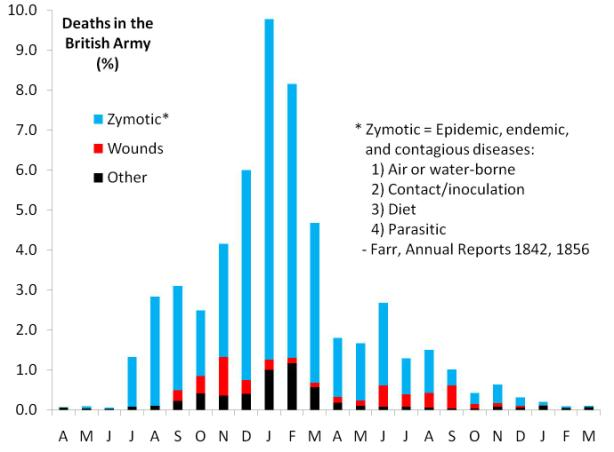
\includegraphics[width=\linewidth,height=0.8\textheight,keepaspectratio]{figures/ng_diagram2.jpg}
\subcaption{Gráfico de barras.}
\end{minipage}
\hfill
\begin{minipage}[t]{0.49\textwidth}
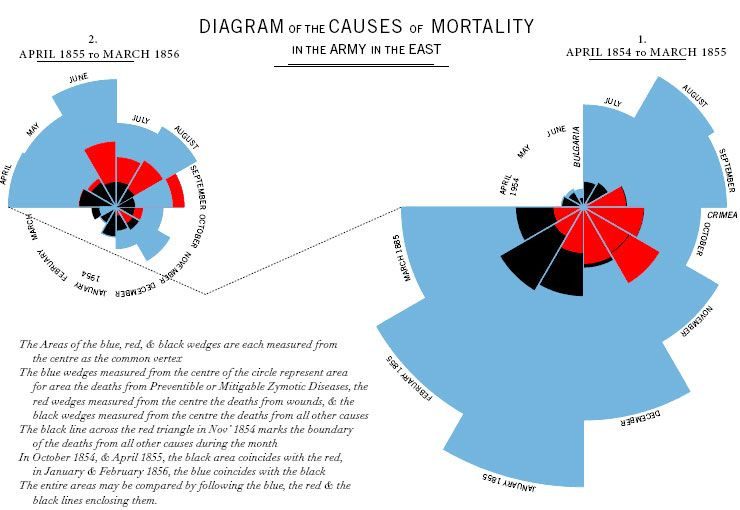
\includegraphics[width=\linewidth,height=0.8\textheight,keepaspectratio]{figures/ng_diagram1.jpg}
\subcaption{Diagrama de Florence Nightingale (\emph{coxcomb plots}).}
\end{minipage}
\caption{Comparação entre os gráficos de mortalidade utilizando os mesmos dados.}
\end{figure}
\end{frame}
% http://www.florence-nightingale-avenging-angel.co.uk/Nightingale_Hockey_Stick.pdf


\begin{frame}[allowframebreaks]
\frametitle{Florence Nightingale no R - \emph{coxcomb diagram}}
\begin{figure}[h]
 \centering
 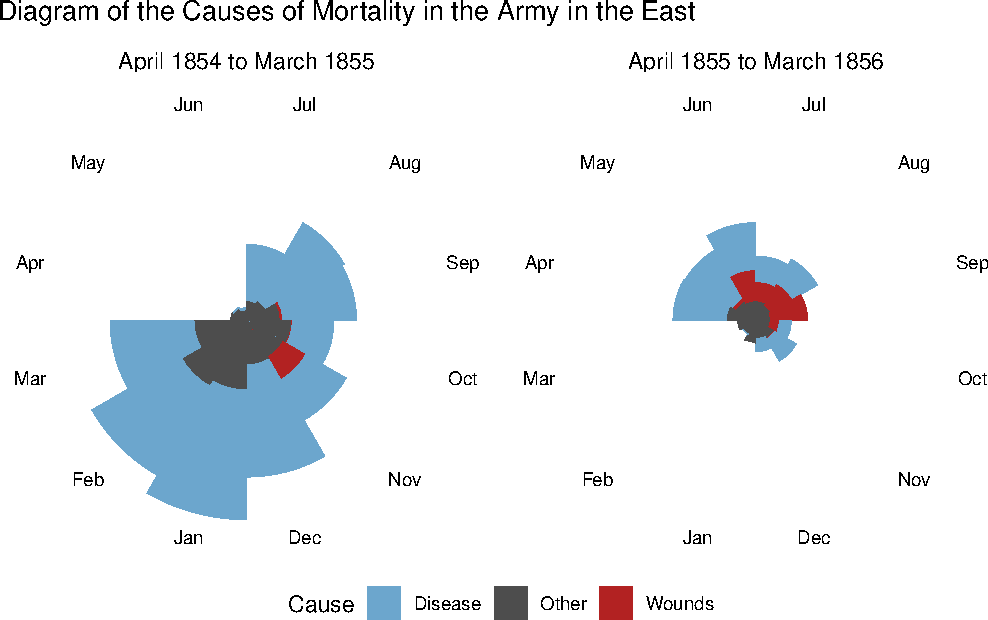
\includegraphics[width=0.8\textwidth,height=0.65\textheight,keepaspectratio]{figures/nightingale-R.pdf}
 \caption{\small Reprodução do gráfico de Florence Nightingale usando \texttt{ggplot2}. Fonte: \url{https://www.r-bloggers.com/2021/03/florence-nightingales-rose-charts-and-others-in-ggplot2/}.}
 \label{fig-nightingale-R}
\end{figure}

\framebreak

\lstinputlisting[language=R, label=lst-nightingale, postbreak=\mbox{$\hookrightarrow$\space}, basicstyle=\fontsize{8}{10}\selectfont\ttfamily]{examples/nightingale-rbloggers.R}

\end{frame}


\begin{frame}[allowframebreaks=1,fragile]
\frametitle{Mortes no Brasil 2003 a 2021}
\begin{minipage}[b]{0.47\textwidth}
\scriptsize
\begin{table}[h]
\csvstyle{mystyle}{
    tabular=lllH,
    head to column names,
    table head= {Date} & {Year} & {Month} & {Deaths} \\\midrule,
    filter={\value{csvrow}<18}
}
\csvreader[mystyle]{examples/obitos-br.csv}{}{\Date & \Year & \Month & \Deaths}
\caption{\label{tab-obitos-br}Número de óbitos no Brasil.}
\end{table}
\end{minipage}
\begin{minipage}[b]{0.47\textwidth}
\scriptsize
Dados obtidos pelo IBGE e Registro Civil:\\
\url{https://sidra.ibge.gov.br/tabela/2681#resultado} \\
\url{https://transparencia.registrocivil.org.br/registros}
\end{minipage}

\framebreak

\begin{figure}[h]
 \centering
 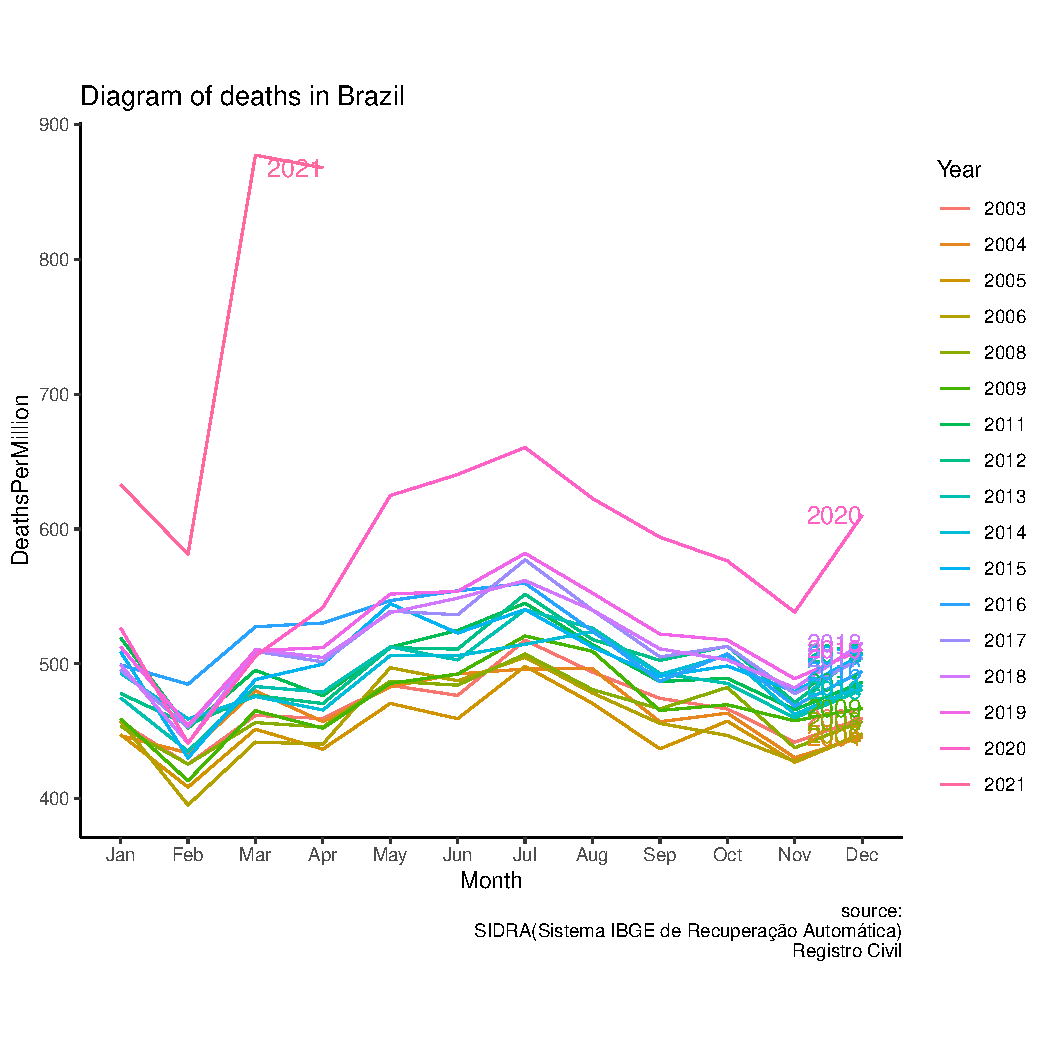
\includegraphics[width=0.8\textwidth,height=0.75\textheight,keepaspectratio]{examples/deaths-brazil-lines-per1E6.pdf}
 \caption{\small Número de óbitos no Brasil de janeiro de 2003 a abril de 2021.}
 \label{fig-deathsbr}
\end{figure}

\framebreak

\begin{figure}[h]
 \centering
 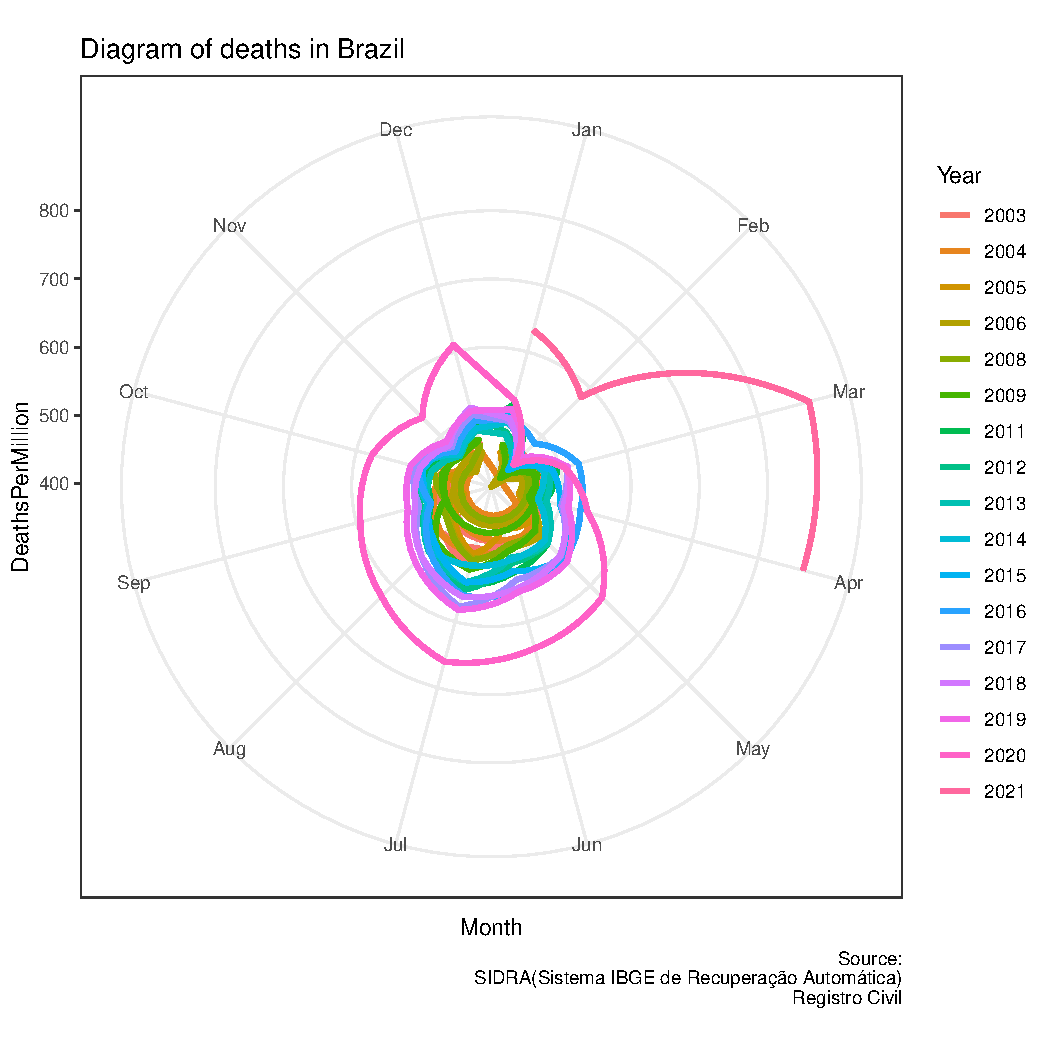
\includegraphics[width=0.8\textwidth,height=0.75\textheight,keepaspectratio]{examples/deaths-brazil-polar-per1E6.pdf}
 \caption{\small Número de óbitos no Brasil de janeiro de 2003 a abril de 2021.}
 \label{fig-deathsbr-polar}
\end{figure}

\framebreak

Carregando as bibliotecas que serão utilizadas:
\lstinputlisting[language=R, label=lst-deathsbr1, linerange={1-3}, postbreak=\mbox{$\hookrightarrow$\space}, basicstyle=\fontsize{8}{10}\selectfont\ttfamily]{examples/deaths-brazil.r}

Preparando os dados:
\lstinputlisting[language=R, label=lst-deathsbr2, linerange={5-13}, postbreak=\mbox{$\hookrightarrow$\space}, basicstyle=\fontsize{8}{10}\selectfont\ttfamily]{examples/deaths-brazil.r}

\framebreak
Gráfico linear:
\lstinputlisting[language=R, label=lst-deathsbr3, linerange={15-21}, postbreak=\mbox{$\hookrightarrow$\space}, basicstyle=\fontsize{8}{10}\selectfont\ttfamily]{examples/deaths-brazil.r}

\framebreak
Gráfico polar:
\lstinputlisting[language=R, label=lst-deathsbr4, linerange={23-31}, postbreak=\mbox{$\hookrightarrow$\space}, basicstyle=\fontsize{8}{10}\selectfont\ttfamily]{examples/deaths-brazil.r}

\end{frame}



\begin{frame}[fragile,allowframebreaks]
\frametitle{Exemplo dados condomínio}
\centering
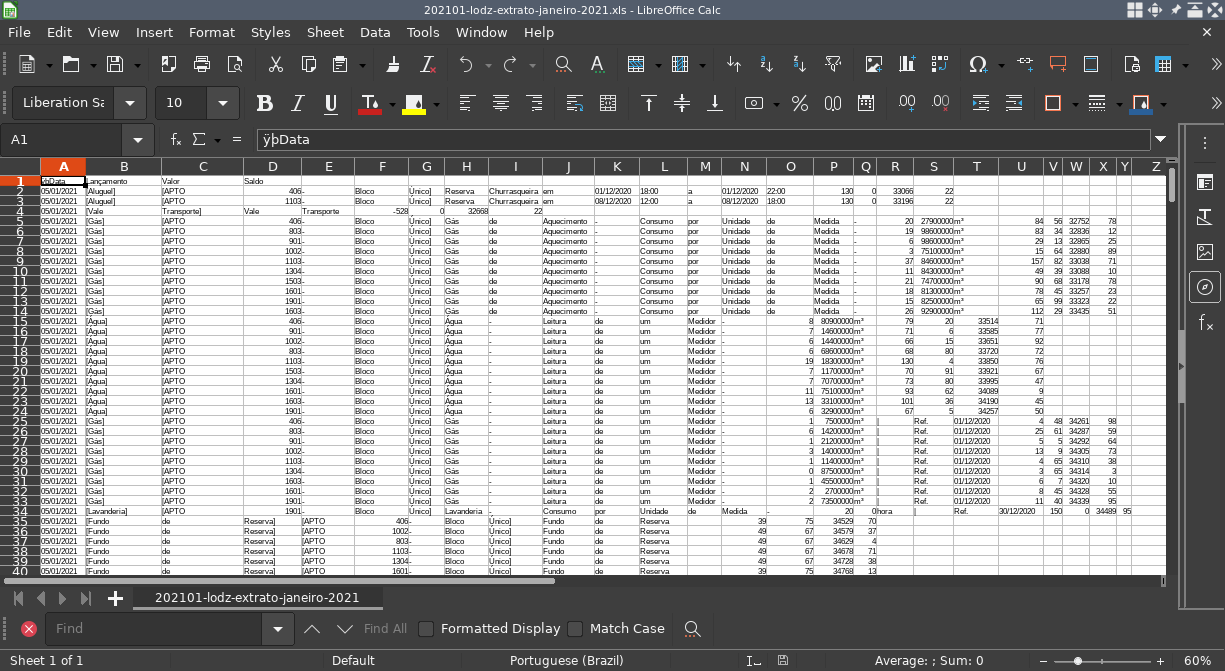
\includegraphics[width=0.8\textwidth,height=0.7\textheight,keepaspectratio]{examples/lodz-planilha-xls.png}

\framebreak
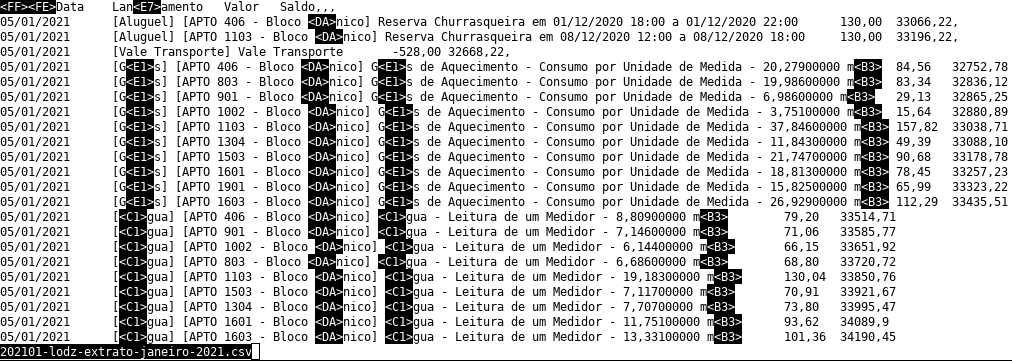
\includegraphics[width=0.8\textwidth,height=0.7\textheight,keepaspectratio]{examples/lodz-planilha-csv.png}

\framebreak
\lstinputlisting[label=lst-lodz-ex-data, postbreak=\mbox{$\hookrightarrow$\space}, basicstyle=\fontsize{5}{7}\selectfont\ttfamily]{examples/datasample.csv}

\framebreak
\lstinputlisting[language=bash, label=lst-lodz-ex-01, postbreak=\mbox{$\hookrightarrow$\space}, basicstyle=\fontsize{8}{10}\selectfont\ttfamily]{examples/analise.sh}

\framebreak
\lstinputlisting[language=bash, label=lst-lodz-ex-02, postbreak=\mbox{$\hookrightarrow$\space}, basicstyle=\fontsize{8}{10}\selectfont\ttfamily]{examples/extractdataall.sh}

\framebreak
\lstinputlisting[language=bash, label=lst-lodz-ex-03, postbreak=\mbox{$\hookrightarrow$\space}, basicstyle=\fontsize{8}{10}\selectfont\ttfamily]{examples/extractdataapto.sh}


\end{frame}



\begin{frame}
Sugestões de leitura: 
\vspace{2ex}

\fullcite{wickhamggplot2}
Disponível em: \url{https://ggplot2-book.org/}

\vspace{3ex}
\fullcite{wilkinson2005grammar}

\vspace{3ex}
From Data to Viz: \url{https://www.data-to-viz.com/}

\vspace{3ex}
The R Graph Gallery: \url{https://www.r-graph-gallery.com/}

\vspace{3ex}
Storytelling with data: \url{https://www.storytellingwithdata.com}\\
/blog, /book, /chart guide

\end{frame}
